\documentclass[border={10pt 5pt 5pt 5pt},tikz]{standalone}

\usepackage[T1]{fontenc}
\usepackage[sfdefault,scaled=.85]{FiraSans}
\usepackage{tikz}
\usepackage{pgfplots}
\usepackage{ifthen}
\usetikzlibrary{arrows.meta}
\usetikzlibrary{shapes.geometric}
\usetikzlibrary{mindmap,trees,shadows}
\pgfplotsset{compat=1.16}

\usetikzlibrary{arrows.meta,angles,quotes}
\colorlet{linecol}{black!75}
\usepackage{forest}

% Information boxes (from : https://texample.net/tikz/examples/servers/)
\newcommand*{\info}[4][5]{%
  \node [ annotation, #3, scale=1.5, text width = #1em,
          inner sep = 1mm ] at (#2) {%
  \list{$\bullet$}{\topsep=0pt\itemsep=0pt\parsep=0pt
    \parskip=0pt\labelwidth=8pt\leftmargin=8pt
    \itemindent=-5pt\labelsep=2pt}%
    #4
  \endlist
  };
}


\begin{document}

	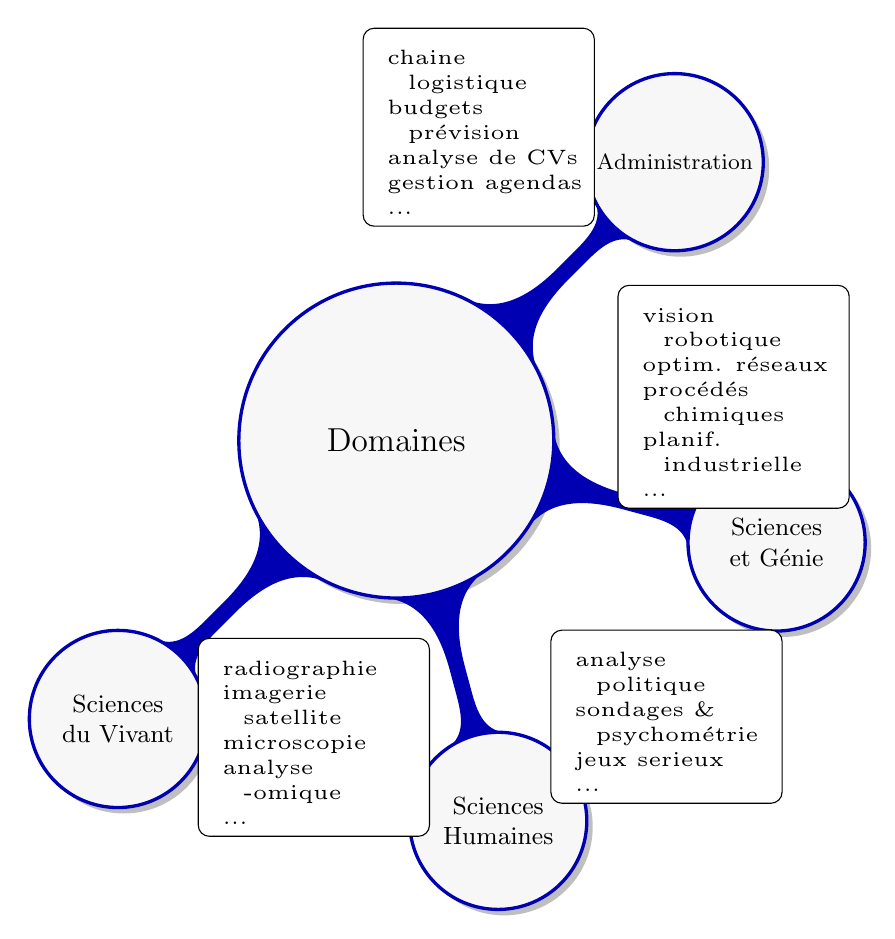
\begin{tikzpicture}[every annotation/.style = {draw, fill = white}]
		\tikzset{concept/.append style={fill={black!3},drop shadow}}
		\path[mindmap,concept color=blue!70!black,text=black]
		% node[concept]{Intelligence Artificielle}
		% [clockwise from=45]
		% child[concept color=green!60!black] {
		% 	node[concept] (data) {Données}
		% 	[clockwise from=180]
		% 	child { node[concept] (tab) {Structurées} }
		% 	child { node[concept] (capt) {Capteurs} }
		% 	child { node[concept] (temp) {Temporelles} }
		% 	child { node[concept] (text) {Textuelles} }
		% 	child { node[concept] (datunc) {Incertaines} }
		% }
		% child[concept color=blue!70!black, sibling angle=72] {
			node[concept] (domains) {Domaines}
			[clockwise from=45]
			child { node[concept,font=\footnotesize] (adm) {Administration} }
			child { node[concept] (sg) {Sciences et Génie} }
			child { node[concept] (sh) {Sciences Humaines} }
			child { node[concept] (sv) {Sciences du Vivant} }
		% }
		% child[concept color=red!70!black, sibling angle=72] {
		% 	node[concept] (objs) {Objectifs}
		% 	[clockwise from=-25]
		% 	child { node[concept] (dec) {Décrire} }
		% 	child[sibling angle=50] { node[concept] (pred) {Prédire} }
		% 	child[sibling angle=50] { node[concept] (opt) {Optimiser} }
		% 	child[sibling angle=50] { node[concept] (pres) {Prescrire} }
		% }
		% child[concept color=purple!70!black, sibling angle=72] { 
		% 	node[concept] (models) {Modèles} 
		% 	[clockwise from=-30]
		% 	child { node[concept] {Graphiques} }
		% 	child[concept color=gray] { 
		% 		node[concept, font=\footnotesize] (ml) {Apprentissage Automatique} 
		% 		[clockwise from=-100]
		% 		child { node[concept] (sup) {Supervisé} }
		% 		child { node[concept] (nsup) {Non-supervisé} }
		% 		child { node[concept] (rl) {Par Renforcement} }
		% 	}
		% 	child { node[concept] (se) {Systèmes Experts} }
		% 	child { node[concept] (stat) {Statistiques} }
		% }
		% child[concept color=yellow!70!black, sibling angle=68] { 
		% 	node[concept] (theory) {Théorie} 
		% 	[clockwise from=-90]
		% 	child { node[concept] (expl) {Explicabilité} }
		% 	child { node[concept] (rob) {Robustesse} }
		% 	child { node[concept] (theunc) {Incertitude} }
		% 	child { node[concept] (cert) {Certification} }
		% 	child { node[concept] (eth) {Éthique} }
		% }
		;
		\info{adm.north west}{above,anchor=east,yshift=-1em}{%
		\item[] chaine logistique
		\item[] budgets prévision
		\item[] analyse de CVs
		\item[] gestion agendas
  		\item[] ...
		}
		\info{sg.north east}{above,anchor=east,xshift=1em,yshift=3em}{%
		\item[] vision robotique
		\item[] optim. réseaux
		\item[] procédés chimiques
  		\item[] planif. industrielle
		\item[] ...
		}
		\info{sh.north east}{above,anchor=west,xshift=-1em,yshift=1.5em}{%
		\item[] analyse politique
		\item[] sondages \& psychométrie
		\item[] jeux serieux
		\item[] ...
		}
		\info{sv.south east}{above,anchor=west,yshift=1.6em}{%
		\item[] radiographie
		\item[] imagerie satellite
		\item[] microscopie
  		\item[] analyse -omique
		\item[] ...
		}
\end{tikzpicture}

\end{document}
